% !TeX program = xelatex
\documentclass[a4paper,10pt]{article}

% ============================================================================
% កញ្ចប់បណ្ណាល័យ (Packages) – អនុវិទ្យាល័យព្រះក្រសាំង (គ្មាន LCD / សន្លឹកកិច្ចការជាគោល)
% ============================================================================
\usepackage[a4paper, left=0.95cm, right=0.95cm, top=0.85cm, bottom=0.92cm, footskip=0.52cm]{geometry}
\usepackage{amsmath}
\usepackage{unicode-math}
\usepackage{fontspec}
\usepackage{array, longtable, multirow, colortbl}
\usepackage[table]{xcolor}
\usepackage{enumitem}
\usepackage{pifont}
\usepackage{fancyhdr}
\usepackage{tikz}
\usetikzlibrary{calc, arrows.meta, decorations.pathreplacing, patterns, positioning, babel}

\makeatletter
\let\@expl@@@mark@update@singlecol@structures@@\relax
\makeatother

% ============================================================================
% ការកំណត់ពុម្ពអក្សរ (Cross-Platform Windows + Linux Cloud fonts/)
% ============================================================================
\providecommand{\NGSFindFonts}{%
  \IfFileExists{C:/Windows/Fonts/cambria.ttc}{%
    \def\NGSSysPath{C:/Windows/Fonts/}%
    \def\NGSUserPath{C:/Users/KIT/AppData/Local/Microsoft/Windows/Fonts/}%
  }{%
    \IfFileExists{./fonts/KhmerOSsiemreap.ttf}{\def\NGSSysPath{./fonts/}\def\NGSUserPath{./fonts/}}{%
    \IfFileExists{../fonts/KhmerOSsiemreap.ttf}{\def\NGSSysPath{../fonts/}\def\NGSUserPath{../fonts/}}{%
    \IfFileExists{../../fonts/KhmerOSsiemreap.ttf}{\def\NGSSysPath{../../fonts/}\def\NGSUserPath{../../fonts/}}{%
    \IfFileExists{../../../fonts/KhmerOSsiemreap.ttf}{\def\NGSSysPath{../../../fonts/}\def\NGSUserPath{../../../fonts/}}{%
    \IfFileExists{../../../../fonts/KhmerOSsiemreap.ttf}{\def\NGSSysPath{../../../../fonts/}\def\NGSUserPath{../../../../fonts/}}{%
    \IfFileExists{../../../../../fonts/KhmerOSsiemreap.ttf}{\def\NGSSysPath{../../../../../fonts/}\def\NGSUserPath{../../../../../fonts/}}{%
    \IfFileExists{../../../../../../fonts/KhmerOSsiemreap.ttf}{\def\NGSSysPath{../../../../../../fonts/}\def\NGSUserPath{../../../../../../fonts/}}{%
      \def\NGSSysPath{../../../../../../../fonts/}\def\NGSUserPath{../../../../../../../fonts/}%
    }}}}}}}%
  }%
}
\NGSFindFonts

\setmathfont[
  Path={\NGSSysPath},
  FontIndex=1,
  Scale=1.02
]{cambria.ttc}

\defaultfontfeatures{Ligatures=TeX}

\setmainfont[
  Path={\NGSUserPath},
  Extension=.ttf,
  Script=Khmer,
  BoldFont={KhmerOSsiemreap},
  BoldFeatures={FakeBold=1.8},
  ItalicFont={KhmerOSsiemreap},
  ItalicFeatures={FakeSlant=0.25},
  BoldItalicFont={KhmerOSsiemreap},
  BoldItalicFeatures={FakeBold=1.8, FakeSlant=0.25}
]{KhmerOSsiemreap}

\newfontfamily\muol[
  Path={\NGSUserPath},
  Extension=.ttf,
  Script=Khmer
]{KhmerOSmuollight}

\newfontfamily\TimesEn[
  Path={\NGSSysPath},
  Extension=.ttf,
  Scale=1.00,
  BoldFont={timesbd},
  ItalicFont={timesi},
  BoldItalicFont={timesbi}
]{times}

\newfontfamily\NagaBold[
  Path={\NGSUserPath},
  Extension=.ttf
]{AKbalthom Naga Bold}

\newfontfamily\CalibriFont[
  Path={\NGSSysPath},
  Extension=.ttf
]{calibri}

\newfontfamily\Tacteing[
  Path={\NGSUserPath}
]{TACTENG.TTF}

\newfontfamily\CourierBullet[
  Path={\NGSSysPath},
  Extension=.ttf
]{cour}
\newcommand{\wcirc}{{\CourierBullet\fontsize{9.5pt}{11pt}\selectfont o}}

\XeTeXlinebreaklocale "km"
\XeTeXlinebreakskip = 0pt plus 1pt minus 0.1pt

% ============================================================================
% ការកំណត់ពណ៌ និងទម្រង់ទំព័រ (Colors & Page Style)
% ============================================================================
\definecolor{stepgray}{HTML}{D9D9D9}
\definecolor{headgray}{HTML}{F2F2F2}
\definecolor{boxgray}{HTML}{D9D9D9}
\definecolor{darkred}{HTML}{C00000}
\definecolor{red5e}{HTML}{FF0000}

\pagestyle{fancy}
\fancyhf{}
\renewcommand{\headrulewidth}{0pt}
\fancyfoot[R]{\CalibriFont\fontsize{11pt}{13pt}\selectfont\thepage}

\setlength{\parindent}{0pt}
\setlength{\parskip}{0pt}
\setlength{\tabcolsep}{3.8pt}

\newcolumntype{L}[1]{>{\raggedright\arraybackslash}p{#1}}

% ============================================================================
% ម៉ាក្រូជំនួយ (Helper Macros)
% ============================================================================
\newcommand{\en}[1]{{\TimesEn #1}}
\newcommand{\enbf}[1]{{\TimesEn\textbf{#1}}}
\newcommand{\unit}[1]{\,\text{\en{#1}}}
\newcommand{\riel}{\,\text{៛}}
\newcommand{\fiveE}[1]{{\NagaBold\fontsize{9.5pt}{13pt}\selectfont\textcolor{red5e}{#1}}}
\newcommand{\timenote}[1]{\textcolor{darkred}{\textit{#1}}}
\newcommand{\redsub}[1]{\textcolor{darkred}{#1}}
\newcommand{\graybox}[1]{\colorbox{boxgray}{\strut\hspace{2pt}#1\hspace{2pt}}}
\newcommand{\ditem}{\tikz[baseline=-0.5ex]\fill (0,0.42ex) -- (0.42ex,0) -- (0,-0.42ex) -- (-0.42ex,0) -- cycle;\hspace{0.3em}}
\newcommand{\cnum}[1]{{\fontsize{10.5pt}{12pt}\selectfont\ding{\numexpr181+#1\relax}}\hspace{0.15em}}
\newcommand{\cfig}[1]{\par\vspace{3pt}{\centering #1\par}\vspace{3pt}}
\newcommand{\stepheader}[1]{\multicolumn{3}{|c|}{\cellcolor{stepgray}\muol #1} \\* \noalign{\hrule height 0.4pt}}
\newcommand{\fboxb}[1]{\begingroup\setlength{\fboxsep}{1.5pt}\fbox{#1}\endgroup}
\newcommand{\khmflourish}{{\Tacteing\fontsize{36pt}{14pt}\selectfont\raisebox{-5pt}{3}}}

% ============================================================================
% ម៉ាក្រូគូសរូប TikZ ស-ខ្មៅ ១០០% (x=1cm, y=1cm, font=\scriptsize, width=7.55cm)
% ============================================================================

% ១. E1 Engage: បេសកកម្មជីកស្រះទឹកសហគមន៍ (អន្ទាក់គុណខ្វែងសមាមាត្រស្រប)
\newcommand{\figEngagePROPThreeOneThree}{%
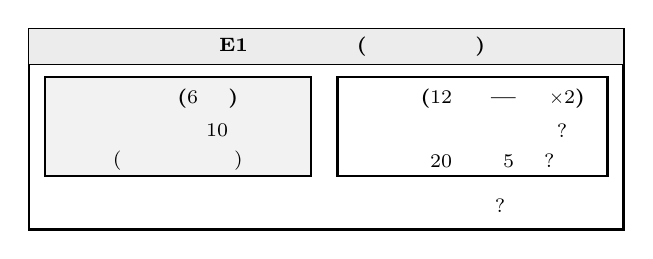
\begin{tikzpicture}[x=1cm, y=1cm, every node/.style={font=\scriptsize, text=black}]
  \draw[black, line width=0.9pt] (0,0) rectangle (7.55,2.55);
  \fill[gray!15] (0,2.10) rectangle (7.55,2.55);
  \draw[black, line width=0.6pt] (0,2.10) -- (7.55,2.10);
  \node at (3.775,2.325) {\textbf{បេសកកម្ម \en{E1}៖ ជីកស្រះទឹកសហគមន៍ (ស្ទង់អន្ទាក់គុណខ្វែង)}};

  \draw[black, line width=0.8pt, fill=gray!10] (0.20,0.68) rectangle (3.58,1.94);
  \node at (1.89,1.66) {\textbf{ក្រុមទី ១ ($6$ នាក់)}};
  \node at (1.89,1.26) {ជីកស្រះដដែលរួចក្នុង \textbf{$10$ ថ្ងៃ}};
  \node at (1.89,0.88) {(ការងារសរុបថេរ ១ ស្រះ)};

  \draw[black, line width=0.85pt] (3.92,0.68) rectangle (7.35,1.94);
  \node at (5.635,1.66) {\textbf{ក្រុមទី ២ ($12$ នាក់ — កើន $\times 2$)}};
  \node at (5.635,1.26) {តើជីកស្រះដដែលរួចក្នុងប៉ុន្មានថ្ងៃ?};
  \node at (5.635,0.88) {ស្មាន៖ \textbf{$20$ ថ្ងៃ} ឬ \textbf{$5$ ថ្ងៃ}?};

  \node at (3.775,0.30) {\textbf{សំណួរគន្លឹះ៖} មនុស្សជួយកាន់តែច្រើន តើចំនួនថ្ងៃត្រូវ\textbf{កើនឡើង} ឬ\textbf{ថយចុះ}?};
\end{tikzpicture}}

% ២. E2 Act 1: ដីចតុកោណកែងមានផ្ទៃក្រឡាថេរ S = 36 m^2 (ទំ.៣០-៣១)
\newcommand{\figExploreAreaPROPThreeOneThree}{%
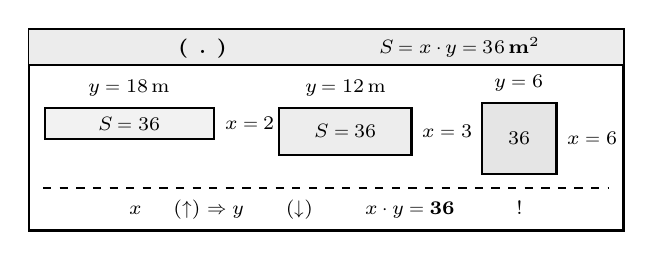
\begin{tikzpicture}[x=1cm, y=1cm, every node/.style={font=\scriptsize, text=black}]
  \draw[black, line width=0.9pt] (0,0) rectangle (7.55,2.55);
  \fill[gray!15] (0,2.10) rectangle (7.55,2.55);
  \draw[black, line width=0.6pt] (0,2.10) -- (7.55,2.10);
  \node at (3.775,2.325) {\textbf{សកម្មភាព ១ (ទំ.៣០)៖ រាងចតុកោណកែងផ្ទៃក្រឡាថេរ $S = x \cdot y = 36\unit{m}^2$}};

  % 2x18 -> scaled
  \draw[black, line width=0.8pt, fill=gray!10] (0.20,1.16) rectangle (2.35,1.56);
  \node at (1.275,1.36) {$S=36$};
  \node[above=0.5pt] at (1.275,1.56) {$y=18\unit{m}$};
  \node[right=0.5pt] at (2.35,1.36) {$x=2$};

  % 3x12 -> scaled
  \draw[black, line width=0.8pt, fill=gray!14] (3.18,0.96) rectangle (4.86,1.56);
  \node at (4.02,1.26) {$S=36$};
  \node[above=0.5pt] at (4.02,1.56) {$y=12\unit{m}$};
  \node[right=0.5pt] at (4.86,1.26) {$x=3$};

  % 6x6 -> scaled
  \draw[black, line width=0.8pt, fill=gray!20] (5.75,0.72) rectangle (6.70,1.62);
  \node at (6.225,1.17) {$36$};
  \node[above=0.5pt] at (6.225,1.62) {$y=6$};
  \node[right=0.5pt] at (6.70,1.17) {$x=6$};

  \draw[black, line width=0.55pt, dashed] (0.18,0.54) -- (7.37,0.54);
  \node at (3.775,0.26) {$x$ កើន ($\uparrow$) $\Rightarrow y$ ថយចុះ ($\downarrow$) តែផលគុណ $x\cdot y = \mathbf{36}$ ថេរជានិច្ច!};
\end{tikzpicture}}

% ៣. E2 Act 2: តារាងប្រៀបធៀប សមាមាត្រស្រប ទល់នឹង សមាមាត្រច្រាស (Sorting Matrix)
\newcommand{\figSortingMatrixPROPThreeOneThree}{%
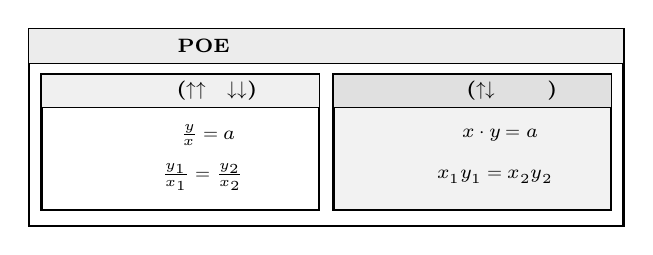
\begin{tikzpicture}[x=1cm, y=1cm, every node/.style={font=\scriptsize, text=black}]
  \draw[black, line width=0.9pt] (0,0) rectangle (7.55,2.50);
  \fill[gray!15] (0,2.06) rectangle (7.55,2.50);
  \draw[black, line width=0.6pt] (0,2.06) -- (7.55,2.06);
  \node at (3.775,2.28) {\textbf{\en{POE} ញែកដាច់៖ សមាមាត្រស្រប ទល់នឹង សមាមាត្រច្រាស}};

  \draw[black, line width=0.8pt] (0.16,0.20) rectangle (3.68,1.92);
  \fill[gray!12] (0.16,1.50) rectangle (3.68,1.92);
  \draw[black, line width=0.55pt] (0.16,1.50) -- (3.68,1.50);
  \node at (1.92,1.71) {\textbf{សមាមាត្រស្រប ($\uparrow\uparrow$ ឬ $\downarrow\downarrow$)}};
  \node at (1.92,1.15) {\textbf{ផលចែកថេរ៖} $\frac{y}{x} = a$};
  \node at (1.92,0.62) {សមីការ៖ $\frac{y_1}{x_1} = \frac{y_2}{x_2}$};

  \draw[black, line width=0.95pt, fill=gray!10] (3.87,0.20) rectangle (7.39,1.92);
  \fill[gray!24] (3.87,1.50) rectangle (7.39,1.92);
  \draw[black, line width=0.6pt] (3.87,1.50) -- (7.39,1.50);
  \node at (5.63,1.71) {\textbf{សមាមាត្រច្រាស ($\uparrow\downarrow$ ផ្ទុយទិស)}};
  \node at (5.63,1.15) {\textbf{ផលគុណថេរ៖} $x\cdot y = a$};
  \node at (5.63,0.62) {សមីការ៖ $x_1 y_1 = x_2 y_2$};
\end{tikzpicture}}

% ៤. E4 Elaborate: គំរូកម្មករ 35 -> 28 នាក់ សង់ផ្ទះ (ទំ.៣១) + ច្រកត្រួតពិនិត្យភាពសមហេតុផល
\newcommand{\figElaborateWorkersPROPThreeOneThree}{%
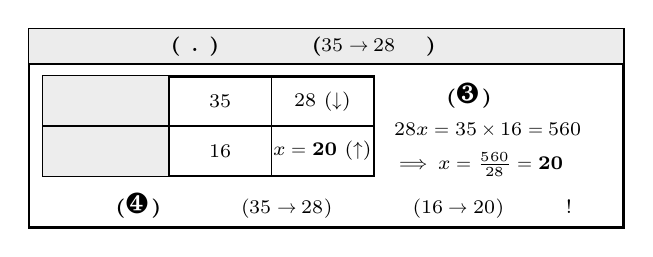
\begin{tikzpicture}[x=1cm, y=1cm, every node/.style={font=\scriptsize, text=black}]
  \draw[black, line width=0.9pt] (0,0) rectangle (7.55,2.52);
  \fill[gray!15] (0,2.08) rectangle (7.55,2.52);
  \draw[black, line width=0.6pt] (0,2.08) -- (7.55,2.08);
  \node at (3.775,2.30) {\textbf{គំរូទី ១ (ទំ.៣១)៖ តារាងផលគុណថេរ ($35 \to 28$ នាក់) និងការផ្ទៀងផ្ទាត់}};

  % តារាងខាងឆ្វេង
  \draw[black, line width=0.8pt] (0.18,0.66) rectangle (4.38,1.92);
  \fill[gray!14] (0.18,0.66) rectangle (1.78,1.92);
  \draw[black, line width=0.6pt] (0.18,1.29) -- (4.38,1.29);
  \draw[black, line width=0.6pt] (1.78,0.66) -- (1.78,1.92);
  \draw[black, line width=0.6pt] (3.08,0.66) -- (3.08,1.92);

  \node at (0.98,1.605) {\textbf{ចំនួនកម្មករ}};
  \node at (0.98,0.975) {\textbf{ចំនួនថ្ងៃ}};
  \node at (2.43,1.605) {$35$};
  \node at (3.73,1.605) {$28$ ($\downarrow$)};
  \node at (2.43,0.975) {$16$};
  \node at (3.73,0.975) {$x = \mathbf{20}$ ($\uparrow$)};

  % គណនាខាងស្ដាំ
  \node[anchor=west] at (4.52,1.68) {\textbf{ផលគុណថេរ (\cnum{3})៖}};
  \node[anchor=west] at (4.52,1.25) {$28x = 35\times 16 = 560$};
  \node[anchor=west] at (4.52,0.80) {$\implies x = \frac{560}{28} = \mathbf{20}$ ថ្ងៃ};

  \node at (3.775,0.28) {\textbf{ផ្ទៀង (\cnum{4})៖} កម្មករថយចុះ ($35\to 28$) ចំនួនថ្ងៃកើន ($16\to 20$) ត្រឹមត្រូវ!};
\end{tikzpicture}}

% ៥. E5 Evaluate: ជម្រើសវិនិច្ឆ័យ A-D
\newcommand{\figExitPROPThreeOneThree}{%
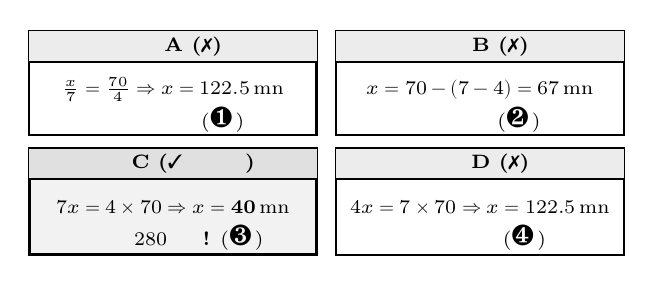
\begin{tikzpicture}[x=1cm, y=1cm, every node/.style={font=\scriptsize, text=black}]
  % A
  \draw[black, line width=0.8pt] (0,1.52) rectangle (3.65,2.84);
  \fill[gray!15] (0,2.45) rectangle (3.65,2.84);
  \draw[black, line width=0.55pt] (0,2.45) -- (3.65,2.45);
  \node at (1.825,2.645) {\textbf{ជម្រើស \en{A} (\ding{55})}};
  \node at (1.825,2.10) {$\frac{x}{7} = \frac{70}{4} \Rightarrow x = 122.5\unit{mn}$};
  \node at (1.825,1.72) {ច្រឡំសមាមាត្រស្រប (\cnum{1})};

  % B
  \draw[black, line width=0.8pt] (3.90,1.52) rectangle (7.55,2.84);
  \fill[gray!15] (3.90,2.45) rectangle (7.55,2.84);
  \draw[black, line width=0.55pt] (3.90,2.45) -- (7.55,2.45);
  \node at (5.725,2.645) {\textbf{ជម្រើស \en{B} (\ding{55})}};
  \node at (5.725,2.10) {$x = 70 - (7-4) = 67\unit{mn}$};
  \node at (5.725,1.72) {ដកថេរខុសក្បួន (\cnum{2})};

  % C (Correct)
  \draw[black, line width=1.1pt, fill=gray!10] (0,0) rectangle (3.65,1.35);
  \fill[gray!24] (0,0.96) rectangle (3.65,1.35);
  \draw[black, line width=0.6pt] (0,0.96) -- (3.65,0.96);
  \node at (1.825,1.155) {\textbf{ជម្រើស \en{C} (\ding{51} ត្រឹមត្រូវ)}};
  \node at (1.825,0.61) {$7x = 4\times 70 \Rightarrow x = \mathbf{40\unit{mn}}$};
  \node at (1.825,0.22) {\textbf{ផលគុណថេរ $280$ ត្រូវ!} (\cnum{3})};

  % D
  \draw[black, line width=0.8pt] (3.90,0) rectangle (7.55,1.35);
  \fill[gray!15] (3.90,0.96) rectangle (7.55,1.35);
  \draw[black, line width=0.55pt] (3.90,0.96) -- (7.55,0.96);
  \node at (5.725,1.155) {\textbf{ជម្រើស \en{D} (\ding{55})}};
  \node at (5.725,0.61) {$4x = 7\times 70 \Rightarrow x = 122.5\unit{mn}$};
  \node at (5.725,0.22) {គូផលគុណខុសជួរឈរ (\cnum{4})};
\end{tikzpicture}}

% ============================================================================
% ចាប់ផ្ដើមឯកសារ (Document Body)
% ============================================================================
\begin{document}
\fontsize{10pt}{15.2pt}\selectfont

% -------------------- ក្បាលកិច្ចតែងការ (Header) --------------------
\begin{center}
  {\muol\fontsize{11pt}{16pt}\selectfont ព្រះរាជាណាចក្រកម្ពុជា}\\[2pt]
  {\muol\fontsize{10pt}{15pt}\selectfont ជាតិ សាសនា ព្រះមហាក្សត្រ}\\[1pt]
  \khmflourish
\end{center}

\vspace{-24pt}
{\muol\fontsize{9.5pt}{12.5pt}\selectfont
មន្ទីរអប់រំ យុវជន និងកីឡា ខេត្តកំពង់ធំ\\
ការិយាល័យអប់រំ យុវជន និងកីឡា ស្រុកកំពង់ស្វាយ\\
អនុវិទ្យាល័យព្រះក្រសាំង}

\vspace{1pt}
\begin{center}
  {\muol\fontsize{10pt}{14pt}\selectfont កិច្ចតែងការបង្រៀន}
\end{center}
\vspace{0pt}

% -------------------- ព័ត៌មានទូទៅ (Metadata) --------------------
{\renewcommand{\arraystretch}{0.98}
\hspace*{3.1cm}%
\begin{tabular}{@{}l l L{11.0cm}@{}}
  - \hspace{0.35cm} មុខវិជ្ជា & : & គណិតវិទ្យា ថ្នាក់ទី៨ (ពីជគណិត) \\
  - \hspace{0.35cm} ចំណងជើងមេរៀន & : & មេរៀនទី៣៖ ទំហំសមាមាត្រនិងភាគរយ \\
  - \hspace{0.35cm} ចំណងជើងរង & : & ១.៣. ទំហំសមាមាត្រច្រាស (ទំ.៣០–៣១, ៤១) \\
  - \hspace{0.35cm} រយៈពេល & : & ១ ម៉ោងសិក្សា (៥០ នាទី) \\
  - \hspace{0.35cm} បង្រៀនដោយ & : & ហុក ប៊ុនថែន \\
  - \hspace{0.35cm} កាលបរិច្ឆេទ & : & ថ្ងៃព្រហស្បតិ៍ ទី១៩ ខែវិច្ឆិកា ឆ្នាំ២០២៦ \\
\end{tabular}

\vspace{2pt}

% -------------------- I. វត្ថុបំណង --------------------
\textbf{I.} {\muol វត្ថុបំណង}\\[1pt]
\hspace*{0.55cm}%
\begin{tabular}{@{}l l L{14.2cm}@{}}
  \wcirc \hspace{0.25cm} វិជ្ជាសម្បទា & : & សិស្សប្រាប់និយមន័យទំហំសមាមាត្រច្រាស រូបមន្តទូទៅ $xy = a$ ឬ $y = \frac{a}{x}$ ($a \neq 0$ ជាមេគុណសមាមាត្រច្រាស) និងប្រាប់លក្ខណៈខុសគ្នារវាងសមាមាត្រស្រប (ផលចែកថេរ) និងសមាមាត្រច្រាស (ផលគុណថេរ) បានត្រឹមត្រូវ ។ \\
  \wcirc \hspace{0.25cm} បំណិនសម្បទា & : & សិស្សបំពេញតារាងផលគុណថេរលើសន្លឹកកិច្ចការ បង្កើតសមីការ $x_1 y_1 = x_2 y_2$ និងដោះស្រាយចំណោទសមាមាត្រច្រាសក្នុងជីវភាពពិត (ផ្ទៃក្រឡាចតុកោណកែង កម្មករសង់ផ្ទះ និងរ៉ូប៊ីនេបញ្ចូលទឹក ទំ.៣០–៣១) បានត្រឹមត្រូវ ។ \\
  \wcirc \hspace{0.25cm} ចរិយាសម្បទា & : & សិស្សមានទម្លាប់ពិនិត្យទិសដៅបម្រែបម្រួលទំហំ ($\uparrow\downarrow$) និងភាពសមហេតុផលនៃចម្លើយមុននឹងសន្និដ្ឋាន មិនគុណខ្វែងតាមទម្លាប់ងងឹតងងល់ និងចេះសហការការងារជាក្រុមក្នុងសហគមន៍ ។ \\
\end{tabular}

\vspace{2pt}

% -------------------- II. សម្ភារៈឧបទេស --------------------
\textbf{II.} {\muol សម្ភារៈឧបទេស}\\[1pt]
\hspace*{0.55cm}$\bullet$ \hspace{0.35cm} សៀវភៅសិក្សាគោលថ្នាក់ទី៨ (ទំ.៣០–៣១, ៤១) ក្ដារខៀន ដីស/ហ្វឺត បន្ទាត់ត្រង់ និង\textbf{សន្លឹកកិច្ចការសិស្សបំពេញចន្លោះ ស-ខ្មៅ} (\en{Printable\_Materials\_PROP313} ទំព័រ ១–២ សម្រាប់សិស្ស និងទំព័រ ៣ ប្លង់ក្ដារខៀន/ចម្លើយគ្រូ — គ្មានប្រើ \en{LCD})

\vspace{2pt}

% -------------------- III. វិធីសាស្រ្តបង្រៀន --------------------
\textbf{III.} {\muol វិធីសាស្រ្តបង្រៀន}\\[1pt]
\hspace*{0.45cm}%
\begin{tabular}{@{}l l L{14.85cm}@{}}
  $\bullet$ \hspace{0.25cm} គោលវិធី & : & សិស្សមជ្ឈមណ្ឌល (សន្លឹកកិច្ចការបំពេញចន្លោះជាគោល + ការពិភាក្សាជាក្រុមតូច ៣ នាក់) \\
  $\bullet$ \hspace{0.25cm} យុទ្ធវិធីបង្រៀន & : & គំរូស្ថាបនានិយម \en{5Es} រួមបញ្ចូល \textbf{តារាងផលគុណថេរ (\en{Constant-Product Table})}, \textbf{\en{POE} បំបែកអន្ទាក់គុណខ្វែង} និង \textbf{តារាងញែកករណីស្រប–ច្រាស (\en{Contrasting Matrix})} \\
\end{tabular}
}

\vspace{2pt}

% -------------------- IV. ដំណើរការបង្រៀន --------------------
\textbf{IV.} {\muol ដំណើរការបង្រៀន}

\vspace{1pt}
{\renewcommand{\arraystretch}{1.12}
\begin{longtable}{|L{5.50cm}|L{7.90cm}|L{4.80cm}|}
\hline
\multicolumn{1}{|c|}{\cellcolor{headgray}\muol សកម្មភាពគ្រូ} &
\multicolumn{1}{c|}{\cellcolor{headgray}\muol ខ្លឹមសារមេរៀន} &
\multicolumn{1}{c|}{\cellcolor{headgray}\muol សកម្មភាពសិស្ស} \\
\endhead
\hline
\endfoot

% ==================== ជំហានទី១ (2min) ====================
\stepheader{ជំហានទី១ \enbf{(}រដ្ឋបាលថ្នាក់\enbf{)}}
$\bullet$ ពិនិត្យវត្តមាន អនាម័យ និងសណ្ដាប់ធ្នាប់ថ្នាក់រៀន \par
$\bullet$ រៀបចំក្រុមតូច ៣ នាក់តាមតុ និងចែក\textbf{សន្លឹកកិច្ចការសិស្ស (\en{PROP313} ទំព័រ ១–២)}
&
$\bullet$ រដ្ឋបាលថ្នាក់ អនាម័យ និងវិន័យសិក្សា \par
$\bullet$ ចែកសន្លឹកកិច្ចការម្នាក់ ១ សន្លឹក សម្រាប់បំពេញតាមដំណាក់កាល \en{E1--E5}
&
$\circ$ ប្រធានថ្នាក់រាយការណ៍វត្តមានសិស្ស \par
$\circ$ ទទួលសន្លឹកកិច្ចការ សរសេរឈ្មោះ និងអង្គុយតាមក្រុម ៣ នាក់ \\
\hline

% ==================== ជំហានទី២ (9min: កំណែ <=3m + រំលឹក 3m + E1 3m) ====================
\stepheader{ជំហានទី២ \enbf{(}កិច្ចការផ្ទះ \enbf{+} ទំនាក់ទំនងមេរៀនថ្មី\enbf{)}}
\ditem \textbf{កំណែកិច្ចការផ្ទះ ($\le\text{\enbf{3\,min}}$)} \par
$\bullet$ ហៅសិស្ស ២ នាក់ឡើងកែលំហាត់ ទំ.៤០ លេខ ២(ក) និងទំ.៤១ លេខ ១១ លើក្ដារខៀន
&
{\centering\redsub{កំណែកិច្ចការផ្ទះមេរៀនមុន (ទំ.៤០ \#2 ក និង ទំ.៤១ \#11)}\par}
$\bullet$ \textbf{\#2 ក៖} $\frac{a}{5} = \frac{b}{18} = \frac{a+b}{5+18} = \frac{138}{23} = 6 \implies b = 18\times 6 = \mathbf{108}$ \par
$\bullet$ \textbf{\#11៖} $\frac{A}{14} = \frac{B}{16} = \frac{C}{18},\; A=105\,000\riel \implies \frac{105\,000}{14}=7\,500\riel$ \par
\hspace*{0.3cm}$\Rightarrow B = 120\,000\riel,\; C = 135\,000\riel,\; \text{សរុប } \mathbf{360\,000\riel}$
&
$\circ$ ផ្ទៀងចម្លើយ និងកែតម្រូវចូលសៀវភៅកិច្ចការផ្ទះ \\[3pt]

\ditem \textbf{រំលឹកមេរៀនទាក់ទង (\enbf{3min})} \par
$\bullet$ សួររំលឹក៖ «ក្នុងសមាមាត្រស្រប $y = ax$ ($a>0$) បើ $x$ កើន ២ ដង តើ $y$ ប្រែប្រួលដូចម្ដេច? ហើយផលអ្វីដែលស្មើតម្លៃថេរ $a$?»
&
{\centering\redsub{រំលឹកទំហំសមាមាត្រស្រប (១.១–១.២)}\par}
$\bullet$ ក្នុងសមាមាត្រស្រប៖ ពេល $x$ កើន ($\uparrow$) នោះ $y$ ក៏កើន ($\uparrow$) ក្នុងផលធៀបដូចគ្នា ហើយ\textbf{ផលចែក $\frac{y}{x} = a$ ថេរជានិច្ច} ។
&
$\circ$ ឆ្លើយ៖ «$y$ កើន ២ ដងដែរ ហើយផលចែក $\frac{y}{x} = a$ ថេរ!» \\[3pt]

\fiveE{E1 - Engage (3min)} \timenote{(កុំទាន់ផ្ដល់ចម្លើយ)} \par
\ditem \textbf{បេសកកម្មជីកស្រះទឹកសហគមន៍ (សន្លឹកកិច្ចការ \en{E1})} \par
$\bullet$ ឱ្យសិស្សអានប្រអប់ \en{E1} ហើយគូសជ្រើសរើសរវាង \textbf{$20$ ថ្ងៃ} និង \textbf{$5$ ថ្ងៃ}
&
\redsub{បេសកកម្ម \en{E1}៖ ជីកស្រះទឹកសហគមន៍} \par
អ្នកភូមិ $6$ នាក់ជីកស្រះទឹកមួយរួចក្នុង $10$ ថ្ងៃ ។ បើអ្នកភូមិកើនដល់ $12$ នាក់ជួយជីកស្រះដដែល សិស្សម្នាក់គុណខ្វែង $\frac{t}{12}=\frac{10}{6} \Rightarrow t=20$ ថ្ងៃ! \par
$\bullet$ តើអ្នកយល់ស្របថាត្រូវការ $20$ ថ្ងៃ ឬត្រូវការតែ $5$ ថ្ងៃ? ហេតុអ្វី?
&
$\circ$ ពិភាក្សាជាគូ និងគូស \ding{51} ក្នុងប្រអប់ \en{E1} លើសន្លឹកកិច្ចការ \\[3pt]

&
\cfig{\figEngagePROPThreeOneThree}
& \\
\hline

% ==================== ជំហានទី៣ (17min: E2 11m + E3 6m) ====================
\stepheader{ជំហានទី៣ \enbf{(}ខ្លឹមសារមេរៀនថ្មី\enbf{)}}
\fiveE{E2 - Explore (11min)} \par
$\bullet$ សរសេរចំណងជើងរង \textbf{១.៣. ទំហំសមាមាត្រច្រាស} លើក្ដារខៀន \par
\ditem \textbf{សកម្មភាព ១៖ តារាងដីចតុកោណកែងផ្ទៃក្រឡាថេរ $36\unit{m}^2$ (\enbf{6min}, សន្លឹកកិច្ចការ \en{E2-A})} \par
$\bullet$ ឱ្យសិស្សបំពេញតារាងទទឹង $x$ បណ្ដោយ $y$ និងជួរផលគុណ $x\cdot y$ (សៀវភៅទំ.៣០–៣១)
&
មេរៀនទី៣ \quad {\muol ទំហំសមាមាត្រនិងភាគរយ \enbf{(}ត\enbf{)}} \par
១.៣. ទំហំសមាមាត្រច្រាស \par
{\centering\textbf{សកម្មភាព ១៖ ដីចតុកោណកែងមានផ្ទៃក្រឡា $S = 36\unit{m}^2$ (ទំ.៣០–៣១)}\par}
{\centering\fontsize{9pt}{12.5pt}\selectfont
\begin{tabular}{|l|c|c|c|c|c|}
\hline
\cellcolor{headgray}ប្រវែងទទឹង $x\ (\text{\en{m}})$ & $1$ & $2$ & $3$ & $4$ & $6$ \\[2pt] \hline
\cellcolor{headgray}ប្រវែងបណ្ដោយ $y\ (\text{\en{m}})$ & $36$ & $18$ & $12$ & $9$ & $6$ \\[2pt] \hline
\cellcolor{headgray}ផលគុណ $x\cdot y$ & $\mathbf{36}$ & $\mathbf{36}$ & $\mathbf{36}$ & $\mathbf{36}$ & $\mathbf{36}$ \\[2pt] \hline
\end{tabular}\par}
&
$\circ$ កត់ចំណងជើងរង រួចបំពេញជួរបណ្ដោយ $y$ និងជួរផលគុណ $x\cdot y$ លើសន្លឹកកិច្ចការ \\[3pt]

$\bullet$ សួរបំផុសឱ្យសិស្សសង្កេតទិសដៅប្រែប្រួលរវាង $x$ និង $y$ និងតម្លៃផលគុណ $xy$
&
$\bullet$ \textbf{ការសង្កេត៖} កាលណាតម្លៃ $x$ កើន ($\uparrow$) តម្លៃ $y$ ថយចុះ ($\downarrow$) ឬពេល $x$ ថយចុះ នោះ $y$ កើន ហើយផលគុណ៖ \par
$xy = 1\times 36 = 2\times 18 = 3\times 12 = 4\times 9 = 6\times 6 = \mathbf{36}$ \par
$\implies xy = 36$ ឬ $y = \dfrac{36}{x}$ ($36$ ជាមេគុណសមាមាត្រច្រាស) ។
&
$\circ$ សន្និដ្ឋាន៖ «$x$ និង $y$ ប្រែប្រួលផ្ទុយទិសគ្នា ហើយផលគុណ $xy=36$ ថេរ!» \\[3pt]

&
\cfig{\figExploreAreaPROPThreeOneThree}
& \\[3pt]

\ditem \textbf{សកម្មភាព ២៖ \en{POE} ញែកករណីស្រប ច្រាស និងបូក (\enbf{5min}, សន្លឹកកិច្ចការ \en{E2-B})} \par
$\bullet$ ឱ្យសិស្សពិនិត្យស្ថានភាពទាំង ៣ ក្នុងប្រអប់ \en{E2-B} រួចគូសញែកប្រភេទទំនាក់ទំនង
&
{\centering\textbf{សកម្មភាព ២៖ \en{POE} តារាងញែកប្រភេទទំនាក់ទំនងទាំង ៣}\par}
$\bullet$ (ក) ទិញសៀវភៅថ្លៃ $800\riel$/ក្បាល៖ $\frac{y}{x} = 800$ $\to$ \textbf{សមាមាត្រស្រប} \par
$\bullet$ (ខ) ជិះកង់ចម្ងាយផ្លូវថេរ $24\unit{km}$៖ $v\cdot t = 24$ $\to$ \textbf{សមាមាត្រច្រាស} \par
$\bullet$ (គ) បងបង្កើតប្អូន $3$ ឆ្នាំ៖ $y - x = 3$ ($xy$ និង $\frac{y}{x}$ មិនថេរ) $\to$ \textbf{មិនសមាមាត្រ!}
&
$\circ$ ពិនិត្យផលចែក និងផលគុណ រួចញែកដាច់រវាង ស្រប ច្រាស និងមិនសមាមាត្រ \\[3pt]

&
\cfig{\figSortingMatrixPROPThreeOneThree}
& \\[3pt]

% --- E3 Explain (6min) ---
\fiveE{E3 - Explain (6min)} \par
$\bullet$ ដឹកនាំសិស្សបង្គុំប្រអប់\textbf{ជាទូទៅ} តាមសៀវភៅគោលទំ.៣១ លើក្ដារខៀន និងសន្លឹកកិច្ចការ \en{E3}
&
$\bullet$ \textbf{ជាទូទៅ (ទំ.៣១)៖} បើ $y$ និង $x$ ជាទំហំសមាមាត្រច្រាស និង $a \neq 0$ ជាមេគុណសមាមាត្រច្រាស នោះគេបាន៖ \par
\hspace*{0.4cm}\graybox{$xy = a \quad \text{ឬ} \quad y = \dfrac{a}{x} \quad (x \neq 0)$} \par
$\bullet$ \textbf{វិបាកសម្រាប់ដោះស្រាយចំណោទ៖} បើ $(x_1, y_1)$ និង $(x_2, y_2)$ ជាគូតម្លៃត្រូវគ្នានៃសមាមាត្រច្រាស នោះ \graybox{$x_1 y_1 = x_2 y_2$} ។
&
$\circ$ បំពេញប្រអប់រូបមន្តទូទៅ និងវិបាក $x_1 y_1 = x_2 y_2$ លើសន្លឹកកិច្ចការ \en{E3} \\[3pt]

$\bullet$ ភ្ជាប់\textbf{ធនាគារហេតុផល \cnum{1}--\cnum{4}} សម្រាប់ការពារអន្ទាក់គុណខ្វែងខុសក្បួន
&
\textbf{ធនាគារហេតុផល (\en{Warrant Bank})៖} \par
\cnum{1} \textbf{ព្រួញទិសដៅផ្ទុយ ($\uparrow\downarrow$)៖} មួយកើន មួយថយក្នុងផលធៀបច្រាសគ្នា \par
\cnum{2} \textbf{ផលគុណថេរ៖} $xy = a \iff y = \frac{a}{x}$ ($a \neq 0$ ជាបរិមាណការងារ/ទំហំសរុបថេរ) \par
\cnum{3} \textbf{គូផលគុណស្មើគ្នា៖} $x_1 y_1 = x_2 y_2$ (គុណតាមជួរឈរគូត្រូវគ្នា!) \par
\cnum{4} \textbf{ច្រកត្រួតពិនិត្យភាពសមហេតុផល៖} មនុស្សតិច $\to$ ថ្ងៃច្រើន; មនុស្សច្រើន $\to$ ថ្ងៃតិច!
&
$\circ$ ផ្ទៀងលេខកូដ \cnum{1}--\cnum{4} លើសន្លឹកកិច្ចការសម្រាប់ប្រើក្នុង \en{E4}--\en{E5} \\
\hline

% ==================== ជំហានទី៤ (20min: E4 10m + E5 10m) ====================
\stepheader{ជំហានទី៤ \enbf{(}ពង្រីកចំណេះដឹង\enbf{)}}
\fiveE{E4 - Elaborate (10min)} \par
\ditem \textbf{លំហាត់គំរូទី ១៖ កម្មករសង់ផ្ទះ $35 \to 28$ នាក់ (ទំ.៣១)} \par
$\bullet$ ឱ្យសិស្សបំពេញតារាង ២ ជួរ និងអនុវត្ត ៣ ជំហានលើសន្លឹកកិច្ចការ \en{E4}
&
{\muol លំហាត់គំរូទី ១} \textbf{(ទំ.៣១ — កម្មករសង់ផ្ទះ)៖} \par
កម្មករ $35$ នាក់សង់ផ្ទះមួយហើយក្នុង $16$ ថ្ងៃ ។ តើកម្មករ $28$ នាក់សង់ផ្ទះនោះហើយក្នុងប៉ុន្មានថ្ងៃ ($x$)? \par
$\bullet$ \textbf{ជំហាន ១ (\cnum{1})៖} កម្មករថយចុះ ($35 \to 28$) $\implies$ ចំនួនថ្ងៃកើនឡើង (សមាមាត្រច្រាស) \par
$\bullet$ \textbf{ជំហាន ២ (\cnum{3})៖} $28x = 35\times 16 \implies x = \dfrac{35\times 16}{28} = \graybox{$20\text{ ថ្ងៃ}$}$
&
$\circ$ បំពេញតារាង គូសព្រួញទិសដៅផ្ទុយ និងគណនាឃើញ $x = 20$ ថ្ងៃ \\[3pt]

&
\cfig{\figElaborateWorkersPROPThreeOneThree}
& \\[3pt]

\ditem \textbf{លំហាត់គំរូទី ២៖ បំពេញតារាងសមាមាត្រច្រាស និង \en{EIA Looking-Back}} \par
$\bullet$ ឱ្យសិស្សរកមេគុណ $a$ និងបំពេញតារាង $xy = 60$ លើសន្លឹកកិច្ចការ \en{E4}
&
{\muol លំហាត់គំរូទី ២} \textbf{(តារាងសមាមាត្រច្រាស)៖} បើ $x$ និង $y$ សមាមាត្រច្រាស ហើយពេល $x=5$ គេបាន $y=12$៖ \par
$\bullet$ មេគុណសមាមាត្រច្រាស៖ $a = 5\times 12 = \mathbf{60} \implies y = \dfrac{60}{x}$ (\cnum{2}) \par
$\bullet$ ពេល $x=10 \Rightarrow y = \mathbf{6}$;\quad ពេល $y=15 \Rightarrow 15x = 60 \Rightarrow x = \mathbf{4}$ ។
&
$\circ$ គណនា $a=60$ រួចបំពេញ $y=6$ និង $x=4$ លើសន្លឹកកិច្ចការ \\[3pt]

$\bullet$ សួរសំណួរឆ្លុះបញ្ចាំង \textbf{\en{EIA Looking-Back} (30 វិនាទី)}
&
\textbf{\en{EIA Looking-Back}៖} «ក្នុងលំហាត់គំរូទី ១ បើសិស្សម្នាក់ច្រឡំសរសេរ $\frac{x}{28}=\frac{16}{35}$ ឃើញ $x=12.8$ ថ្ងៃ តើយើងដឹងភ្លាមថាខុសដោយសារអ្វី?» ($\to$ ផ្ទុយនឹង \cnum{4}៖ កម្មករតិចជាងមុនមិនអាចសង់ផ្ទះហើយលឿនជាង $16$ ថ្ងៃទេ!)
&
$\circ$ ឆ្លើយ៖ «កម្មករថយចុះ ចំនួនថ្ងៃត្រូវតែធំជាង $16$ ថ្ងៃ!» \\[3pt]

% --- E5 Evaluate (10min) ---
\fiveE{E5 - Evaluate (10min)} \par
\ditem \textbf{ប្រតិបត្តិជាក្រុមតូច ៣ នាក់ (6min, សន្លឹកកិច្ចការ \en{E5})} \par
$\bullet$ ឱ្យសិស្សដោះស្រាយ \textbf{ប្រតិបត្តិទី ១ (រ៉ូប៊ីនេបញ្ចូលទឹក ទំ.៣១)}
&
{\muol លំហាត់ប្រតិបត្តិទី ១} \textbf{(ទំ.៣១ — រ៉ូប៊ីនេបញ្ចូលទឹក)៖} \par
ប្រើរ៉ូប៊ីនេ $4$ ចំណាយពេល $70\unit{mn}$ ពេញអាង ។ បើប្រើរ៉ូប៊ីនេ $7$ តើត្រូវចំណាយពេលប៉ុន្មាននាទី ($x$)? \par
$\bullet$ រ៉ូប៊ីនេកើន ($4\to 7$) $\implies$ រយៈពេលថយចុះ (\cnum{1})៖ \par
\hspace*{0.3cm}$7x = 4\times 70 = 280 \implies x = \dfrac{280}{7} = \graybox{$40\unit{mn}$}$ (\cnum{3}, \cnum{4})
&
$\circ$ បង្កើតសមីការផលគុណថេរ $7x = 4\times 70$ គណនាឃើញ $x = 40\unit{mn}$ \\[3pt]

$\bullet$ បន្ត \textbf{ប្រតិបត្តិទី ២ (ច្រូតស្រូវរួមគ្នា)} និង\textbf{បិទបញ្ចប់បេសកកម្ម \en{E1}}
&
{\muol លំហាត់ប្រតិបត្តិទី ២ និងបិទបេសកកម្ម \enbf{E1}} \textbf{៖} \par
$\bullet$ \textbf{បិទបេសកកម្ម \en{E1}៖} អ្នកភូមិ $12$ នាក់ជីកស្រះរួចក្នុង $12t = 6\times 10 \implies t = \mathbf{5\text{ ថ្ងៃ}}$ (មិនមែន $20$ ថ្ងៃទេ!) \par
$\bullet$ \textbf{ច្រូតស្រូវ៖} កសិករ $15$ នាក់ច្រូតស្រូវរួចក្នុង $12$ ថ្ងៃ ។ បើមាន $20$ នាក់៖ $20x = 15\times 12 = 180 \implies x = \mathbf{9\text{ ថ្ងៃ}}$ ។
&
$\circ$ បិទបេសកកម្ម \en{E1} ($t=5$ ថ្ងៃ) និងគណនាឃើញ $x = 9$ ថ្ងៃ \\[3pt]

\ditem \textbf{សំណួរវិនិច្ឆ័យ \en{A--D} និងសំបុត្រចេញ (4min)} \par
$\bullet$ ឱ្យសិស្សគូសរង្វង់ជម្រើសត្រូវលើសន្លឹកកិច្ចការ រួចលើកម្រាមដៃ ១--៤
&
{\centering\textbf{សំណួរវិនិច្ឆ័យ \en{A--D}៖ រ៉ូប៊ីនេ $4$ ប្រើពេល $70\unit{mn}$ តើរ៉ូប៊ីនេ $7$ ប្រើសមីការណា?}\par}
&
$\circ$ វិភាគជម្រើស \en{A--D} និងលើកម្រាមដៃ ៣ (\textbf{ជម្រើស \en{C}}) \\[3pt]

&
\cfig{\figExitPROPThreeOneThree}
& \\[3pt]

$\bullet$ បញ្ជាក់ចម្លើយត្រូវ (\textbf{ជម្រើស \en{C}}) និងឱ្យបំពេញ\textbf{សំបុត្រចេញ ៦០ វិនាទី}
&
$\bullet$ \textbf{សំបុត្រចេញ៖} បើ $x$ និង $y$ សមាមាត្រច្រាស ហើយ $x=8$ ត្រូវនឹង $y=6$ នោះ៖ (១) មេគុណ $a = 8\times 6 = \mathbf{48}$ (\cnum{2}); (២) បើ $x=12$ នោះ $y = \frac{48}{12} = \mathbf{4}$ (\cnum{3}) ។
&
$\circ$ បំពេញសំបុត្រចេញលើសន្លឹកកិច្ចការមុនបញ្ចប់ម៉ោង \\
\hline

% ==================== ជំហានទី៥ (<=2min) ====================
\stepheader{ជំហានទី៥ \enbf{(}កិច្ចការផ្ទះ \enbf{+} បណ្ដាំផ្ញើ\enbf{)}}
\timenote{ចំណាយពេលឱ្យតិចបំផុតកុំឱ្យលើស 2min} \par
$\bullet$ ណែនាំប្រអប់\textbf{កិច្ចការផ្ទះ}លើសន្លឹកកិច្ចការទំព័រ ២ (សៀវភៅគោល ទំ.៤១ លេខ ៨ និងលេខ ៩)
&
{\centering{\muol កិច្ចការផ្ទះ} \textbf{(សៀវភៅគោល ទំ.៤១៖ លេខ ៨ និង លេខ ៩)}\par} \par
$\bullet$ \textbf{\#8 (ទំ.៤១ — ប្រយ័ត្នញែកប្រភេទ!)៖} កម្មករ $25$ នាក់ដដែល ធ្វើការ $26\unit{h}$ បានស្បែកជើង $1\,300$ គូ ។ បើផលិត $450$ គូ តើត្រូវធ្វើការប៉ុន្មានម៉ោង? \par
\hspace*{0.3cm}($\Rightarrow$ កម្មករថេរ ស្បែកជើងតិច ម៉ោងក៏តិច ជា\textbf{សមាមាត្រស្រប}៖ $\frac{t}{450}=\frac{26}{1\,300} \implies t = \mathbf{9\unit{h}}$)
&
$\circ$ គូសចំណាំលំហាត់ \#8 និងចំណាំពិនិត្យទិសដៅប្រែប្រួលមុនសរសេរសមីការ \\[3pt]

$\bullet$ ណែនាំគន្លឹះលំហាត់ \#9 (ផលគុណម៉ោងការងារសរុបថេរ) និងផ្ដាំផ្ញើអានមេរៀនបន្ទាប់
&
$\bullet$ \textbf{\#9 (ទំ.៤១ — ផលគុណការងារសរុបថេរ)៖} កម្មការិនី $12$ នាក់ $\times 7\unit{h}/\text{ថ្ងៃ} \times 8\text{ ថ្ងៃ}$ ស្មើនឹង $16$ នាក់ $\times x\unit{h}/\text{ថ្ងៃ} \times 16\text{ ថ្ងៃ}$ \par
\hspace*{0.3cm}($\Rightarrow 256x = 672 \implies x = \frac{672}{256} = \mathbf{\frac{21}{8}\unit{h} = 2.625\unit{h}}$ ឬ $2\unit{h}\,37\unit{mn}\,30\unit{s}$) \par
$\bullet$ \textbf{បណ្ដាំផ្ញើ៖} អានមុន \textbf{២.១–២.២ ភាគរយ ប្រាក់ចំណេញនិងប្រាក់ខាត (ទំ.៣១–៣៣)} ។
&
$\circ$ កត់ត្រាបណ្ដាំផ្ញើ ទុកសន្លឹកកិច្ចការក្នុងសៀវភៅ និងជម្រាបលាគ្រូ \\
\end{longtable}

% -------------------- កាលបរិច្ឆេទ និងហត្ថលេខា (Date & Signature) --------------------
\vspace{8pt}
\hfill
\begin{minipage}{10.5cm}
  {\centering
    ថ្ងៃព្រហស្បតិ៍ ១០កើត ខែកត្តិក ឆ្នាំមមី អដ្ឋស័ក ពុទ្ធសករាជ ២៥៧០\\[2pt]
    កំពង់ស្វាយ, ថ្ងៃទី១៩ ខែវិច្ឆិកា ឆ្នាំ២០២៦\\[3pt]
    {\muol គ្រូបង្រៀន}\par}
  \vspace{30pt}
  \hfill{\muol ហុក ប៊ុនថែន}\hspace*{1.4cm}
\end{minipage}

\end{document}
